\chapter{Manipula\c{c}\~ao de arquivos e comandos no sistema}
Manipular arquivos e executar comandos no sistema \'e muito simples em Perl, pode-se criar, editar e excluir arquivos de texto e muitas outras coisas 
interessantes. No exemplo da figura 23 pode-se observar que foi feito o uso do comando \textit{system (''comando do sistema'');}. O comando \textit{system} 
\'e respons\'avel por avisar que o conte\'udo entre parenteses e aspas ser\'a executado diretamente no sistema, sendo assim, os comandos podem variar de SO 
para SO. O comando \textit{mkdir} \'e um comando do sistema Linux que \'e respons\'avel por criar diret\'orios.

\begin{figure}[!htb]
	\centering
	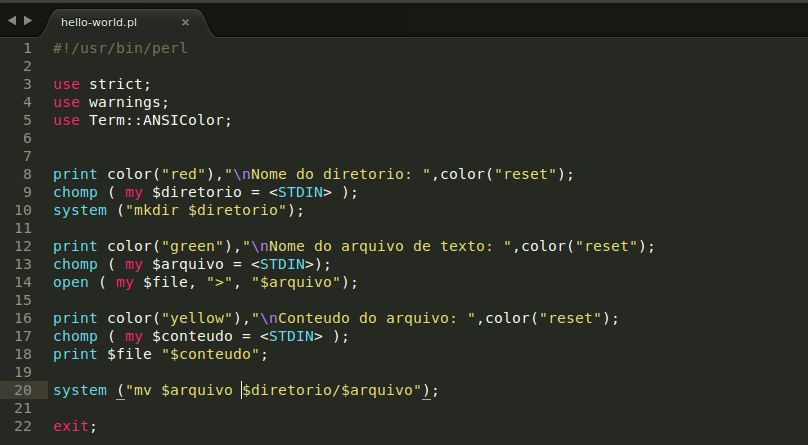
\includegraphics[width=0.5\textwidth]{../5_figuras/image23}
	\caption{Algoritmo executando tarefas no sistema}
\end{figure}

\clearpage

Observa-se o pedido para que o usu\'ario fornecesse o nome do diret\'orio para posteriormente este ser criado, na sequ\^encia \'e requisitado o nome do 
arquivo, sedno criado caso este j\'a n\~ao exista e finalmente \'e requisitado a escrita de conte\'udo deseja que exista no arquivo. J\'a na 20$^a$ linha, 
o arquivo \'e movido para o diret\'orio criado no in\'icio do nosso c\'odigo, um exemplo de sa\'ida pode ser visto na figura 24.

\begin{figure}[!htb]
	\centering
	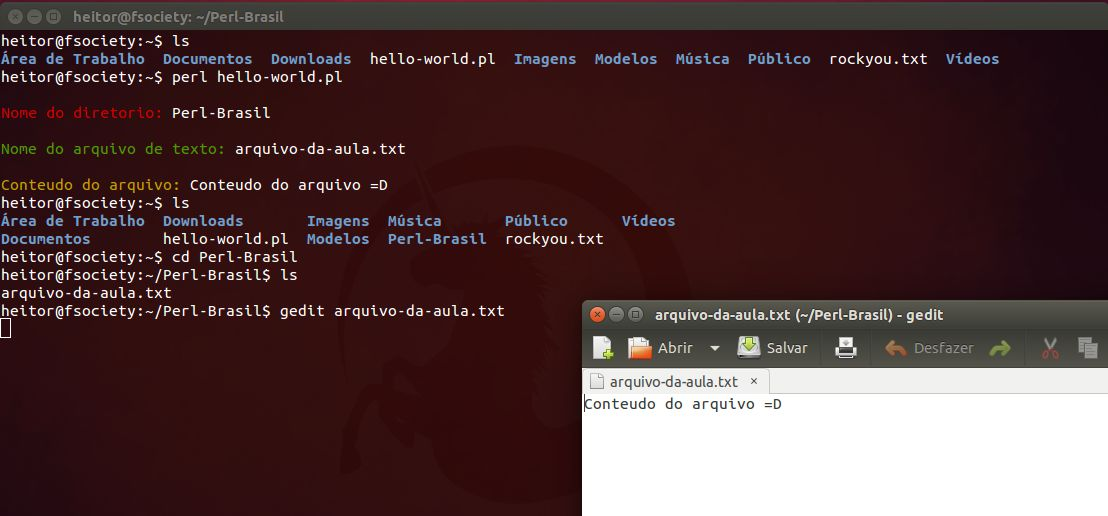
\includegraphics[width=0.8\textwidth]{../5_figuras/image24}
	\caption{Sa\'ida do algoritmo executando tarefas no sistema}
\end{figure}

\begin{itemize}
    \item{\$arquivo: abre ARQUIVO apenas para leitura (o mesmo que \textit{$<$\$arquivo);}}
    \item{\textit{$>$\$arquivo}: abre ARQUIVO para escrita, criando-o caso ainda n\~ao exista}
    \item{\textit{$>>$\$arquivo}: abre ARQUIVO para modificação (append)} 
    \item{\textit{+$>$\$arquivo}: abre ARQUIVO para leitura/escrita. }
\end{itemize}


 